\documentclass[tikz, border=1cm]{standalone}
\usetikzlibrary{shapes}

\begin{document}

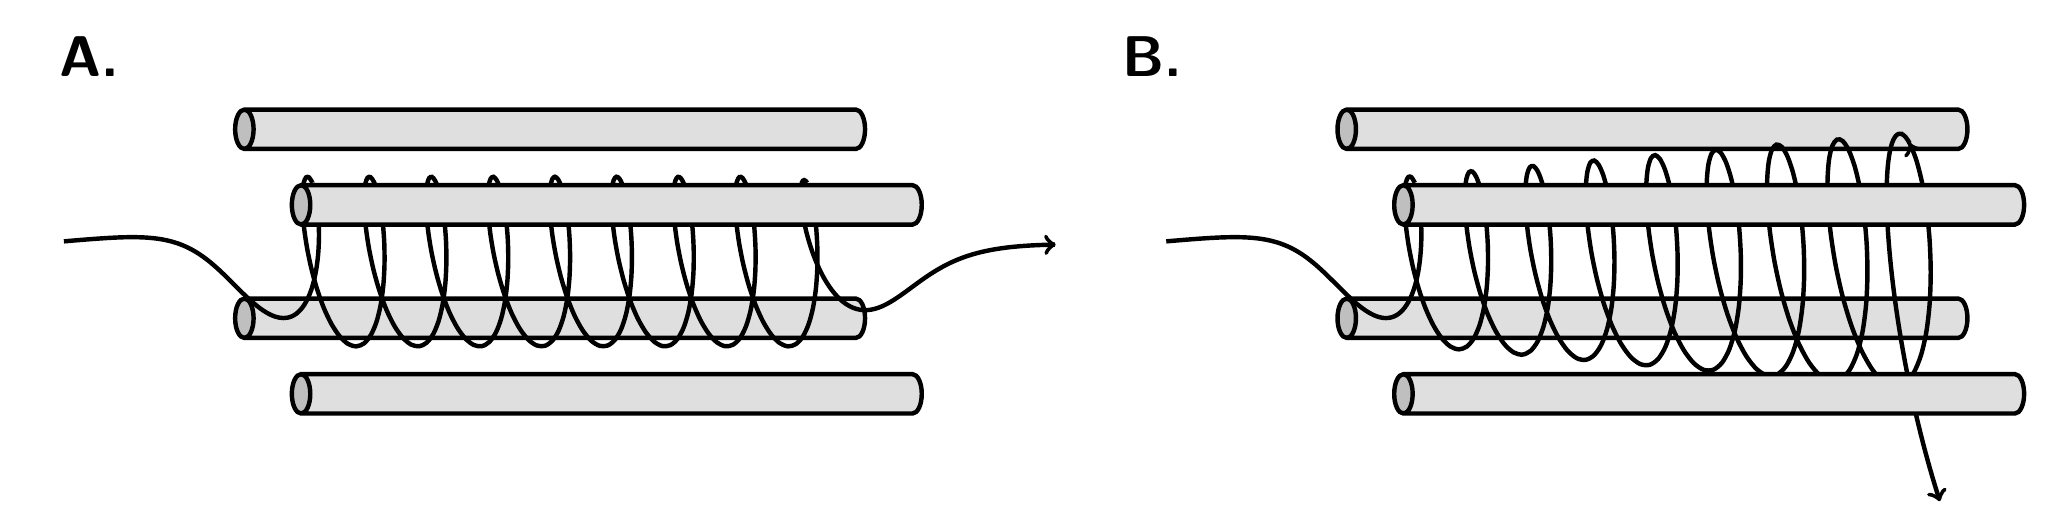
\begin{tikzpicture}[ultra thick, z={(-3mm, 4mm)}]
\newcommand{\mainscale}{1.2}
\newcommand{\pitch}{8}
\newcommand{\domA}{-pi}
\newcommand{\domB}{0}
\newcommand{\domC}{2*pi}
\newcommand{\domD}{3*pi}
\newcommand{\domE}{\domC+pi/\pitch}
\newcommand{\ampA}{(1/(1+\domB-\x))}
\newcommand{\ampB}{(1/(1-\domC+\x))}
\newcommand{\ampC}{(0.08*(\x-\domB)+1)}
\newcommand{\ampD}{(1+((\x-\domC)/(\domE-\domC))^4)}

\tikzset{ mystyle/.style={draw, rotate=180, minimum height=8cm,
    minimum width=5mm, cylinder uses custom fill, cylinder body
    fill=gray!25, cylinder end fill=gray!50},
  arrowstyle/.style = {->, smooth, samples=200},
  font={\fontsize{20pt}{12}\sffamily}
}

\node at (3.5, \mainscale, \mainscale) [cylinder, mystyle]{};
\node at (3.5, -\mainscale, \mainscale) [cylinder, mystyle]{};

\draw[domain={\domA:\domB}, smooth, samples=100] plot (\x, {\ampA*cos((\ampA*\pitch*\x+(1-\ampA)*\pitch*\domB) r)}, {\ampA*sin((\ampA*\pitch*\x+(1-\ampA)*\pitch*\domB) r)}  );
\draw[arrowstyle, domain={\domB:\domC}, smooth, samples=200] plot (\x, {cos(\pitch*\x r)} , {sin(\pitch*\x r)} );
\draw[arrowstyle, domain={\domC:\domD}] plot (\x, {\ampB*cos((\ampB*\pitch*\x+(1-\ampB)*\pitch*\domC) r)}, {\ampB*sin((\ampB*\pitch*\x+(1-\ampB)*\pitch*\domC) r)}  );

\node at (3.5, \mainscale, -\mainscale) [cylinder, mystyle]{};
\node at (3.5, -\mainscale, -\mainscale) [cylinder, mystyle]{};

\node[label=right:{\textbf{A.}}] (n1) at (-3.5, 2.6) {};
\node[label=right:{\textbf{B.}}] (n1) at (10.0, 2.6) {};

\begin{scope}[xshift=14cm]
  \node at (3.5, \mainscale, \mainscale) [cylinder, mystyle]{};
  \node at (3.5, -\mainscale, \mainscale) [cylinder, mystyle]{};

\draw[arrowstyle, domain={\domA:\domB}] plot (\x, {\ampA*cos((\ampA*\pitch*\x+(1-\ampA)*\pitch*\domB) r)}, {\ampA*sin((\ampA*\pitch*\x+(1-\ampA)*\pitch*\domB) r)}  );  
\draw[arrowstyle, domain={\domB:\domC}] plot (\x, {\ampC*cos(\pitch*\x r)} , {\ampC*sin(\pitch*\x r)} );
\draw[arrowstyle, domain={\domC:\domE}] plot (\x, {\ampC*\ampD*cos(\pitch*\x r)} , {\ampC*\ampD*sin(\pitch*\x r)} );

\node at (3.5, \mainscale, -\mainscale) [cylinder, mystyle]{};
\node at (3.5, -\mainscale, -\mainscale) [cylinder, mystyle]{};

\end{scope}

\end{tikzpicture}

\end{document}